\documentclass[tikz,border=0pt]{standalone}
\usepackage{tikz}
\usetikzlibrary{arrows.meta, positioning, shapes.geometric, calc}

% Color palette (matches the styling in the figure)
\definecolor{Garnet}{HTML}{73000A}
\definecolor{CBlue}{HTML}{73000a}
\definecolor{CDark}{HTML}{000000}
\definecolor{CGrayLight}{HTML}{E5E5E5}
\definecolor{CGrayMid}{HTML}{AAAAAA}
\definecolor{CGrayDark}{HTML}{555555}
\definecolor{CWhite}{HTML}{FFFFFF}

\begin{document}

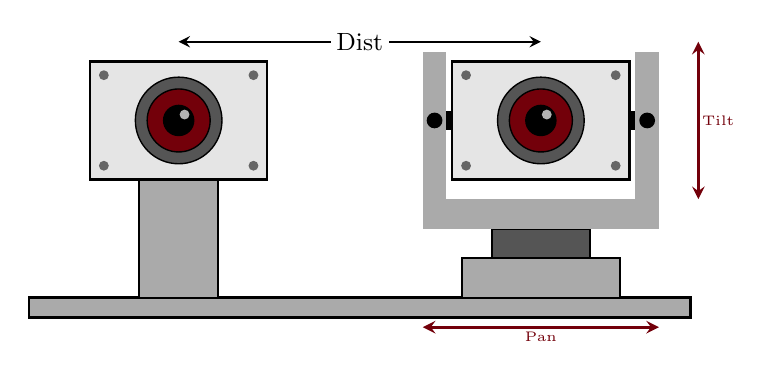
\begin{tikzpicture}[
    scale=1.0,
    % Reusable styles for consistent strokes/fills
    camera body/.style={fill=CGrayLight, draw=black, line width=0.8pt},
    camera dark/.style={fill=CGrayDark, draw=black, line width=0.8pt},
    lens outer/.style={fill=Garnet, draw=black, line width=0.5pt},
    lens inner/.style={fill=black, draw=none},
    mount/.style={fill=CGrayMid, draw=black, line width=0.8pt},
    label text/.style={font=\small, align=center}
]

    % Base rail / platform shared by both camera mounts
    \fill[CGrayMid, draw=black, line width=1pt] (-4.2, 0) rectangle (4.2, 0.25);

    % -------------------------
    % Left: fixed camera module
    % -------------------------
    \begin{scope}[shift={(-2.3, 0.25)}, scale=2.5] % shift places it on the left; scale sizes the module
        \fill[mount] (-0.2, 0) rectangle (0.2, 0.9); % vertical post
        \begin{scope}[shift={(0, 0.90)}] % camera body sits on top of the post
            \fill[camera body] (-0.45, -0.3) rectangle (0.45, 0.3);
            % Corner screws (visual detail only)
            \foreach \x in {-0.38, 0.38}
                \foreach \y in {-0.23, 0.23}
                    \fill[black!60] (\x, \y) circle (0.025);

            % Lens stack (outer housing + red ring + inner aperture + highlight)
            \fill[camera dark, draw=black, line width=0.5pt] (0, 0) circle (0.22);
            \fill[lens outer] (0, 0) coordinate (L1_Center) circle (0.16);
            \fill[lens inner] (0, 0) circle (0.08);
            \fill[white, opacity=0.7] (0.03, 0.03) circle (0.025);

            % Reference point kept in case you later want distance-from-lens measurements
            \coordinate (L1) at (L1_Center);
        \end{scope}
    \end{scope}

    % -----------------------------------
    % Right: pan/tilt camera gimbal module
    % -----------------------------------
    \begin{scope}[shift={(2.3, 0.25)}, scale=2.5] % shift places it on the right; scale sizes the module
        % Base + pedestal under the gimbal
        \fill[mount] (-0.4, 0) rectangle (0.4, 0.2);
        \fill[camera dark] (-0.25, 0.2) rectangle (0.25, 0.35);

        % Gimbal "U" bracket (side uprights + top bar)
        \fill[CGrayMid] (-0.6, 0.35) rectangle (0.6, 0.5);
        \fill[CGrayMid] (-0.6, 0.5) rectangle (-0.48, 1.25);
        \fill[CGrayMid] (0.48, 0.5) rectangle (0.6, 1.25);

        % Small hinge/servo details on the uprights
        \fill[CDark] (-0.48, 0.85) rectangle (-0.42, 0.95);
        \fill[CDark] (0.42, 0.85) rectangle (0.48, 0.95);
        \fill[CDark] (-0.54, 0.9) circle (0.04);
        \fill[CDark] (0.54, 0.9) circle (0.04);

        % Camera head within the gimbal (positioned higher to sit between uprights)
        \begin{scope}[shift={(0, 0.9)}]
            \fill[camera body] (-0.45, -0.3) rectangle (0.45, 0.3);
            \foreach \x in {-0.38, 0.38}
                \foreach \y in {-0.23, 0.23}
                    \fill[black!60] (\x, \y) circle (0.025);
            \fill[camera dark, draw=black, line width=0.5pt] (0, 0) circle (0.22);
            \fill[lens outer] (0, 0) coordinate (L2_Center) circle (0.16);
            \fill[lens inner] (0, 0) circle (0.08);
            \fill[white, opacity=0.7] (0.03, 0.03) circle (0.025);
        \end{scope}

        % Tilt annotation (vertical travel shown next to the gimbal)
        \draw[<->, >=stealth, Garnet, thick, line width=1pt] (0.8, 0.5) -- (0.8, 1.3);
        \node[Garnet, font=\tiny, right] at (0.77, 0.9) {Tilt};

        % Pan annotation (horizontal travel shown under the right module)
        \draw[<->, >=stealth, Garnet, thick, line width=1pt] (-0.6, -0.15) -- (0.6, -0.15);
        \node[Garnet, font=\tiny] at (0, -0.2) {Pan};
    \end{scope}

    % Distance annotation (top arrow spanning between left/right module centers)
    \draw[<->, >=stealth, black, thick] (-2.3, 3.5) -- (2.3, 3.5);
    \node[fill=white, inner sep=2pt, font=\small, text=black] at (0,3.5) {Dist};

\end{tikzpicture}
\end{document}
